todo: move to intro?

The concentric ellipse pair comprises two confocal ellipses. With this choice a miracle happens: any Poncelet trajectory (closed or not) obeys the reflection rule at each vertex: incoming/outgoing rays are bisected by the normal. For this reason this system is known as the {\em Elliptic Billiard},  Figure~\ref{fig:billiard}.

As the only integrable planar billiard \cite{kaloshin2018}, this system has been widely studied. A remarkable invariant of an $N$-periodic billiard family is perimeter \cite{sergei91,connes07}. Experimentally we've also detected the sum of internal angle cosines $\sum\cos{\theta_i}$ is invariant \cite{reznik19} as well as upwards of 40 new invariants \cite{reznik2020-forty} involving angles, lengths, areas, and polygons associated with the N-periodics, about half of which have been proven \cite{akopyan2020-invariants,bialy2020-invariants,caliz2020-area-product}.

\begin{figure}
    \centering
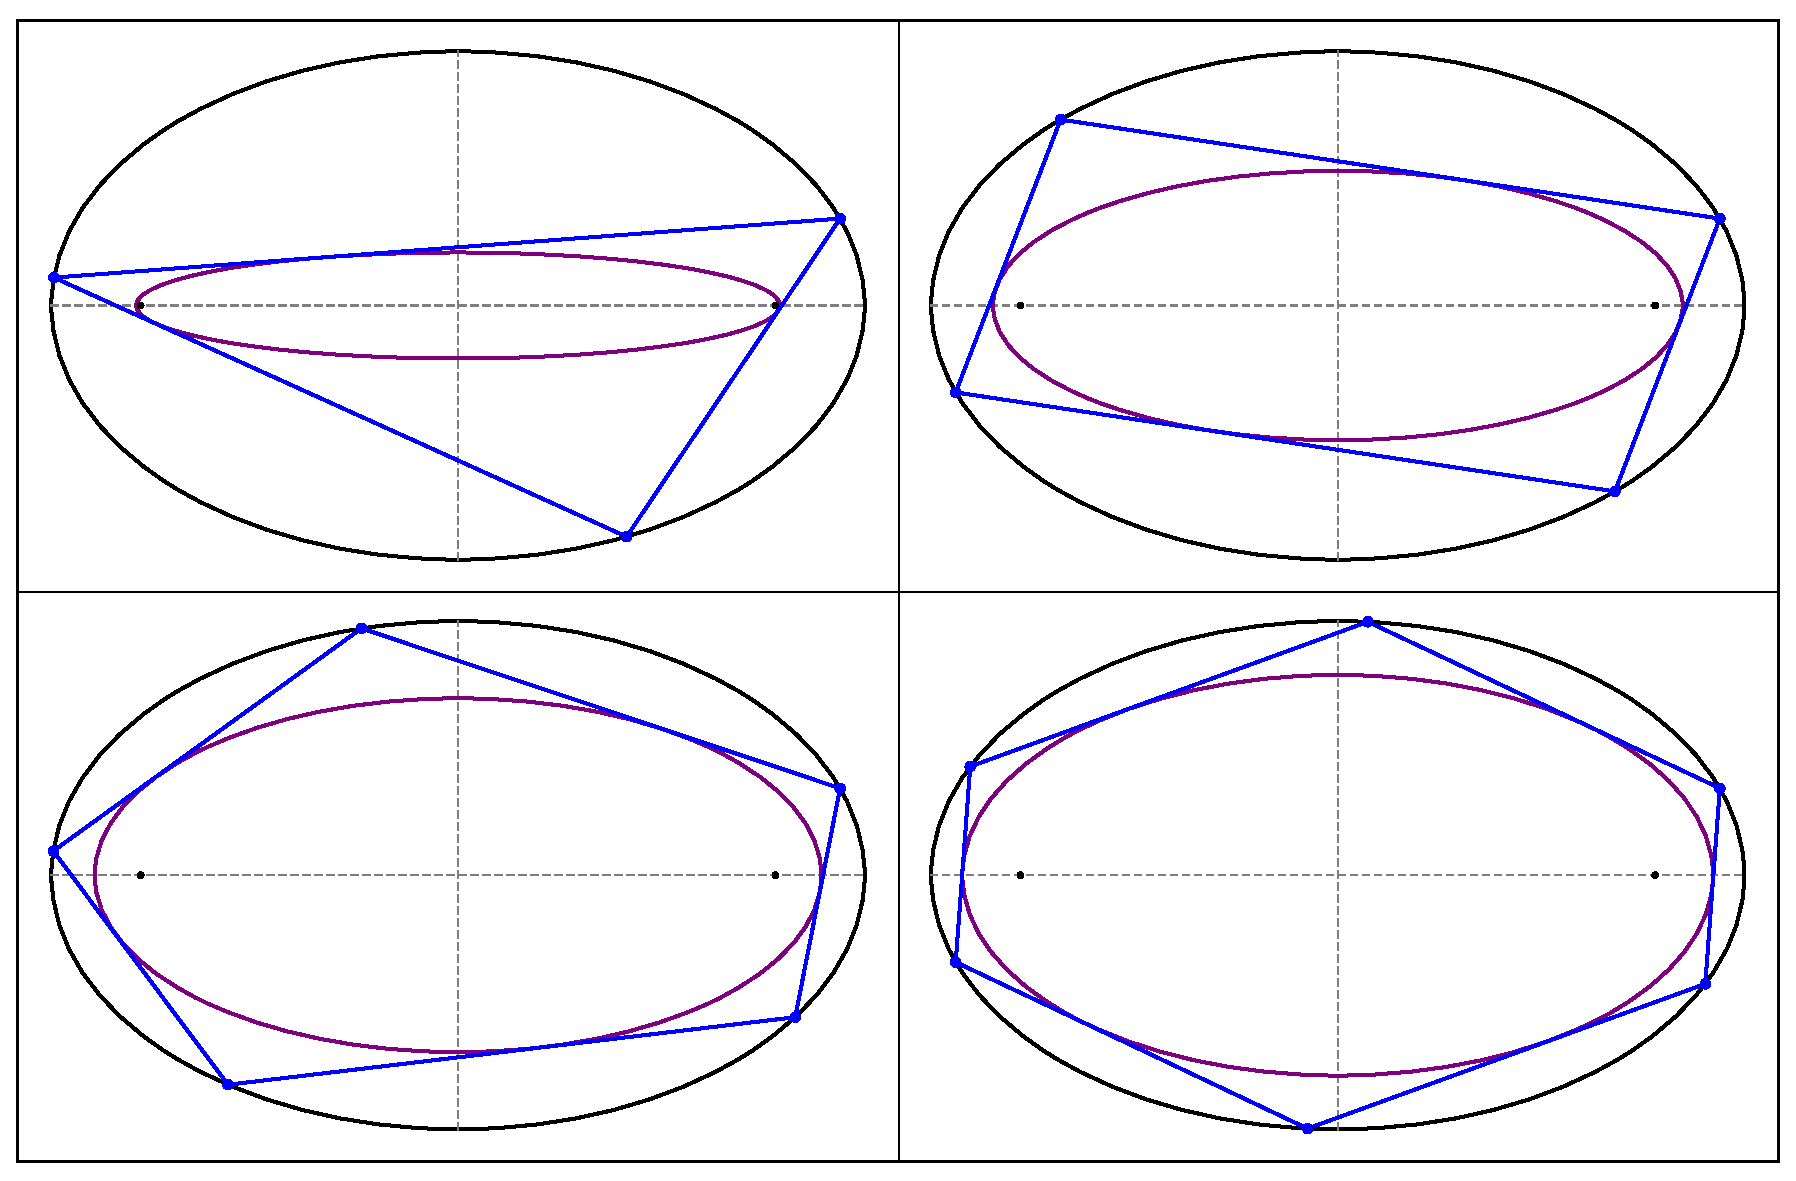
\includegraphics[width=\textwidth]{pics/0050_system_0.eps}
    \caption{N-periodics for a confocal pair (Elliptic Billiard \cite{sergei91}). The reflection rule is obeyed at every vertex, perimeter, sum of cosines, and a slew of 50 other invariants are observed \cite{reznik19,reznik2020-forty}.}
    \label{fig:billiard}
\end{figure}